\subsection{Mesh Partitioning}
\label{subsec:mpi:partitioning}

\todorev{Last revised (with minor changes) on Sat, June 30 at 23:03 by pfac}

In order to distribute processing payload across each process, the input mesh, and all of the data associated with it, needs to be split into partitions.
A mesh partitioning algorithm is required. This algorithm must generate $P$ disjointed partitions (where $P$ is the number of processes), each to be assigned to a different process.
Some additional data is also required for each partition, so that information about how each partition connects to the others is kept, to allow communication to be done correctly.

\subsubsection{Research in Mesh Partitioning}
\label{subsubsec:mpi:partitioning:research}

Mesh partitioning is currently an actively researched topic, with some projects and libraries being already available to help understanding how a mesh (or more generically, a graph) can be partitioned in ways to optimize certain aspects like load balancing, communication balancing or partitioning overhead.
For instance, in \cite{metis}, a library called \texttt{Metis} is presented whose purpose is precisely this problem. Other works found for this topic include \cite{gilbert1995, walshaw2000}.

However, given the already mentioned time constraints of this project, and since the priority was to have a functional algorithm rather than an optimal one, it was decided not to attempt an approach involving \texttt{Metis} or any other researched work.
%Actually, the method used to partition the mesh is quite naive, as shown in \cref{subsubsec:mpi:partitioning:method}.

\subsubsection{Partitioning Methodology}
\label{subsubsec:mpi:partitioning:method}

The algorithm created to partition the mesh works by dividing it in slices by the horizontal coordinate of each cell.
Given a mesh with a total of $C$ cells, and a pool of $P$ processes, the mesh is divided into $P$ partitions, each with exactly $N=C/P$ cells, differing by at most one cell when they cannot be evenly divided.
By ordering the cells based on their horizontal coordinate, they are sequentially assigned to each process, in such a way that the first process receives the first $N$ cells of the set, and so on.

\begin{figure}[!htp]
	\begin{subfigure}[b]{0.5\columnwidth}
		\centering
		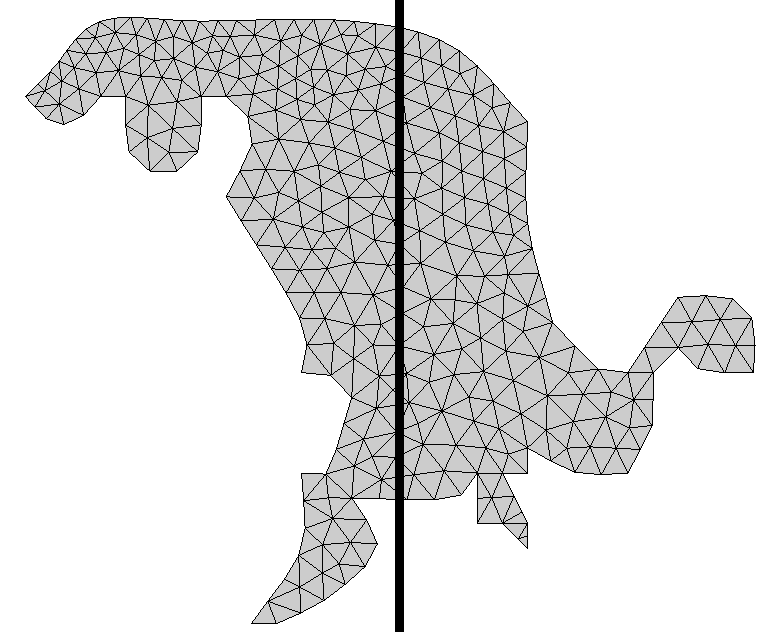
\includegraphics[width=\columnwidth]{foz_p2_msh}
		\caption{2 partitions}
		\label{fig:foz_p2_msh}
	\end{subfigure}%
	\begin{subfigure}[b]{0.5\columnwidth}
		\centering
		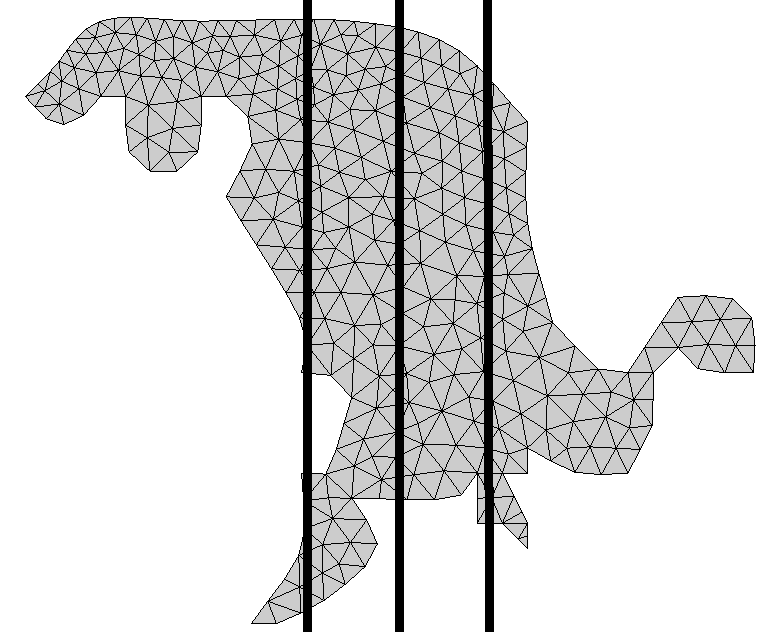
\includegraphics[width=\columnwidth]{foz_p4_msh}
		\caption{4 partitions}
		\label{fig:foz_p4_msh}
	\end{subfigure}%

	\caption{Mesh partitioning illustration}
	\label{fig:partitioning}
\end{figure}

With this partitioning method, communication is also greatly simplified, as it is guaranteed that every partition will have a left and a right neighbor.
It is also assumed that the width of the global mesh is big enough so that there are never processes with no cells assigned, which would break communication.
Since a common mesh usually contains at least thousands of cells, this should not be an issue.
The partitioning and assignment of the cells is done sequentially, thus it will increase preparation time.
